\chapter{Principal Component Analysis} 
\label{appendix-pca} 

Principal component analysis (PCA) is the simplest matrix decomposition model. The PCA model can be formulated as an optimization problem. Given a $N$-by-$M$ matrix $\mathbf{X}$ with $N$ variables and $M$ features, we can approximate $\mathbf{X}$ with the product of two orthogonal rank-one matrices:
\begin{align}
    \mathbf{X} \approx \mathbf{U}\mathbf{V}^T = \sum_{r=1}^R u_r \circ v_r,
\end{align}
where $\circ$ denotes the outer product operator. The equivalent element-wise formulation of the PCA model is
\begin{align}
\label{pca}
    x_{i j} \approx \sum^R_{r = 1} u_i^r v_j^r.
\end{align}
With PCA, the dimensionality of the original matrix can be reduced from from $N$-by-$M$ to $N$-by-$R$. This can be illustrated with the diagram below
\begin{figure}[H]
    \centering
        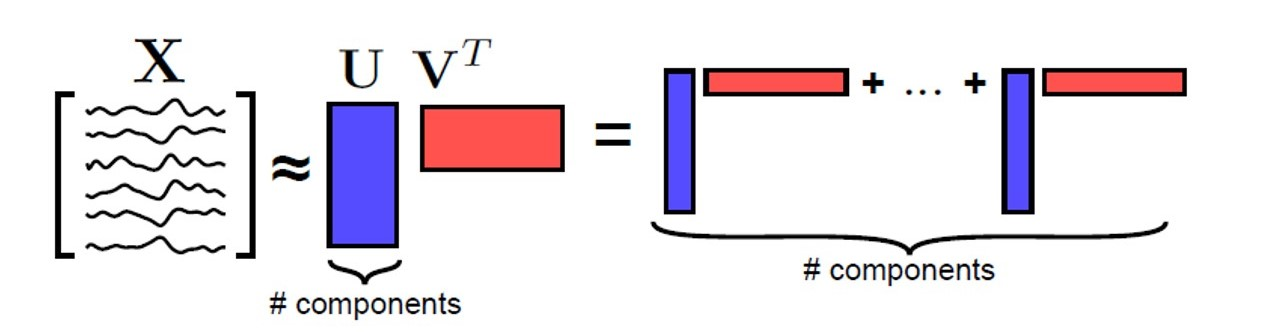
\includegraphics[width=0.7\textwidth]{figures/linear/pca.jpg}
        \caption{Illustration for PCA. (Adapted from \cite{williams_unsupervised_2018})}
    \end{figure} 
PCA seeks to solve a sequence of optimization problems:
\begin{itemize}
    \item maximize variance:
\begin{maxi}|l|
  {\mathbf{V}}{\|\mathbf{X}\mathbf{V}\mathbf{V}^T\|_F^2}{}{}
  \addConstraint{\mathbf{V}\text{ orthonormal}},
 \end{maxi}
 \item minimize residuals:
 \begin{mini}|l|
  {\mathbf{U},\mathbf{V}}{\|\mathbf{X} - \mathbf{U}\mathbf{V}^T\|_F^2}{}{}
  \addConstraint{\mathbf{U,V}\text{ orthogonal}},
 \end{mini}
where $\|\cdot\|_F$ denotes the Frobenius norm.
%  Note that without the constraint of $\mathbf{U},\mathbf{V}$ being orthogonal, PCA has infinite number of solutions since
%  $\mathbf{U}\mathbf{V}^T = \mathbf{U}F^{-1} F\mathbf{V}^T = \mathbf{U}^\prime \mathbf{V}^{\prime T}.$

\end{itemize}

\par When the data has a non-negative constraint, non-negative matrix factorization (NMF) is used. In NMF, the second part of the optimization becomes the following instead:
 \begin{mini}|l|
  {\mathbf{U},\mathbf{V}}{\|\mathbf{X} - \mathbf{U}\mathbf{V}^T\|_F^2}{}{}
  \addConstraint{\mathbf{U}\geq 0, \mathbf{V} \geq 0.}
 \end{mini}
